%% Template for EU deliverable, using the deliverable.sty style file

\documentclass[12pt,a4paper,twoside]{article}

%% common package
\usepackage[headers]{deliverable}
\usepackage{xspace}
\usepackage{verbatim}
\usepackage[usenames]{color}
\usepackage{listings}
\usepackage[usenames,dvipsnames,table]{xcolor}
\usepackage[pdftex,dvips]{graphicx}
\usepackage{url}
\usepackage{array}
%%

%%insert here other packages needed by sections

%%

%%%%%%%%%%%%%%%%%%%%%%%%%%%%%%%%%%%%%%%%%%%%%%%%%%%%%%%%%%%%%%%%%%%%%%%%%%%%%%
%%% Titlepage
%%%%%%%%%%%%%%%%%%%%%%%%%%%%%%%%%%%%%%%%%%%%%%%%%%%%%%%%%%%%%%%%%%%%%%%%%%%%%%

% declaration of variables used in style
\deliverableDocnumber{D1.1}
\deliverableTitle{Enhanced iCub simulator for whole-body contact simulation}

\deliverableAuthor{Vincent Padois$^{1,2}$}
\deliverableResponsiblePartner{UPMC}
\deliverableAffiliation{% Insert here authors affiliations
 $^1$ Sorbonne Universit\'es, UPMC Paris 06, UMR 7222, Institut des Syst\`emes Intelligents et de Robotique (ISIR), F-75005, Paris, France.
 
 $^2$ CNRS, UMR 7222, Institut des Syst\`emes Intelligents et de Robotique (ISIR), F-75005, Paris, France.
}


\deliverableCoordinator{Vincent Padois}
\deliverableActivityNumber{n} %% n=1,..,10
\deliverableActivity{Enhanced iCub simulator for whole-body contact simulation}
\deliverableDoctype{Deliverable} %% or Prototype
\deliverableClassification{Public} % or Consortium
\deliverableDistribution{Consortium} %
\deliverableStatus{Final} % Draft or Final
\deliverableDeliveryDate{28/2/2014}
\deliverableFile{D11\_iCubSimulator.pdf} % please do not use "-" in the name
\deliverableVersion{1.0}
\deliverableDate{Feb.~28, 2014}
\deliverableYear{2014}
\deliverablePages{\pageref{LastPage}}
\deliverableChangelog{}
\deliverableProjectStartingDate{1st March 2013}
\deliverableProjectEndDate{28th February 2017}
\deliverableProjectAcronym{CoDyCo}
\deliverableProjectTitle{Whole-Body Compliant Dynamical Contacts in Cognitive Humanoids}
\deliverableContractNumber{600716}
\deliverableProjectCoordinator{Istituto Italiano di Tecnologia}
\deliverableProjectUrl{www.codyco.eu}
\deliverableFrameworkProgramme{FP7}
 
\deliverableWorkpackage{WP1}
\deliverableEditors{Vincent Padois}
\deliverableContributors{Serena Ivaldi, Mingxing Liu, Vincent Padois (UPMC) / Andrea Del Prete, Francesco Nori, Daniele Pucci, Francesco Romano, Silvio Traversao (IIT) / Leon \v{Z}lajpah (JSI)}

\deliverableAbstract{The work described in this deliverable is part of WP1 and aims at providing the CoDyCo consortium with a shared framework for the simulation of humanoid robots and/or digital humans involved in whole-body and multi-contact activities. In order to reach this goal, several activities have been led in parallel. They are described in this deliverable.}
\deliverableReviewers{}
\deliverableKeywordList{dynamics simulators, humanoid robots, digital human, URDF}

%%%%%%%%%%%%%%%%%%%%%%%%%%%%%%%%%%%%%%%%%%%%%%%%%%%%%%%%%%%%%%%%%%%%%%%%%%%%%%
%%% Sections
%%%%%%%%%%%%%%%%%%%%%%%%%%%%%%%%%%%%%%%%%%%%%%%%%%%%%%%%%%%%%%%%%%%%%%%%%%%%%%

%% constants
\newcommand{\botegoCaps}{BOTEGO}
\newcommand{\certhCaps}{CERTH}
\newcommand{\cybionCaps}{CYBION}
\newcommand{\nuigCaps}{NUIG}
\newcommand{\ubitechCaps}{UBITECH}
%%

%%%%%%%%%%%%%%%%%%%%%%%%%%%%%%%%%%%%%%%%%%%%%%%%%%%%%%%%%%%%%%%%%%%%%%%%%%%%%%
%%% Misc. by Vincent
%%%%%%%%%%%%%%%%%%%%%%%%%%%%%%%%%%%%%%%%%%%%%%%%%%%%%%%%%%%%%%%%%%%%%%%%%%%%%%
\usepackage{titlesec}
\newcommand{\sectionbreak}{}
\graphicspath{{./images/}}
\usepackage{pdfpages}
\usepackage{caption}
\usepackage{subcaption}
\usepackage{slashbox}
\usepackage{multirow}
\usepackage{appendix}
\usepackage{hyperref}
\hypersetup{
    bookmarks=true,         % show bookmarks bar?
    unicode=false,          % non-Latin characters in Acrobat’s bookmarks
    pdftoolbar=true,        % show Acrobat’s toolbar?
    pdfmenubar=true,        % show Acrobat’s menu?
    pdffitwindow=false,     % window fit to page when opened
    pdfstartview={FitH},    % fits the width of the page to the window
    pdftitle={D11\_iCubSimulator.pdf},    % title
    pdfauthor={Vincent Padois},     % author
    pdfsubject={Enhanced iCub simulator for whole-body contact simulation},   % subject of the document
    pdfcreator={Vincent Padois},   % creator of the document
    pdfproducer={Vincent Padois}, % producer of the document
    pdfkeywords= {}, % list of keywords
    pdfnewwindow=true,      % links in new window
    colorlinks=true,       % false: boxed links; true: colored links
    linkcolor=black,          % color of internal links (change box color with linkbordercolor)
    citecolor=black,        % color of links to bibliography
    filecolor=black,      % color of file links
    urlcolor=black           % color of external links
}
\newcommand{\REPORTARXIV}{\href{http://arxiv.org/abs/1402.7050}{http://arxiv.org/abs/1402.7050}}
%%%%%%%%%%%%%%%%%%%%%%%%%%%%%% BEGIN DOCUMENT
\begin{document}

\deliverableMaketitle

%%TODO move to style
\newcolumntype{L}[1]{>{\raggedright\let\newline\\\arraybackslash\hspace{0pt}}m{#1}}
\newcolumntype{C}[1]{>{\centering\let\newline\\\arraybackslash\hspace{0pt}}m{#1}}
\newcolumntype{R}[1]{>{\raggedleft\let\newline\\\arraybackslash\hspace{0pt}}m{#1}}

\textbf{Document Revision History}
\begin{center}
\begin{tabular}{|C{2cm}|C{3cm}|C{5cm}|C{4cm}|}
\hline
\textbf{Version}&\textbf{Date}&\textbf{Description}&\textbf{Author}\\\hline
v.~0.1 & Feb.~20, 2014 & Initial draft & Vincent Padois\\ \hline
v.~0.5 & Feb.~25, 2014 & Intermediate version & Vincent Padois \\ \hline
v.~0.9 & Feb.~27, 2014 & Final version & Vincent Padois \\ \hline
v.~1.0 & Feb.~28, 2014 & Proofread version & Francesco Nori \\ \hline
\end{tabular}
\end{center}
 
 \clearpage

\newpage
\renewcommand*\contentsname{Table of Contents}
\renewcommand*\listfigurename{Index of Figures}
\tableofcontents
\newpage
\listoffigures
\newpage

%%%%%%%%%%%%%%%%%%%%%%%% Start deliverable content here.

\section{Introduction}

The work described in this deliverable is part of WP1 and aims at providing the CoDyCo consortium with a shared framework for the simulation of humanoid robots and/or digital humans involved in whole-body and multi-contact activities. In order to reach this goal, several activities have been led in parallel. They are described in this deliverable as follows. In Section~\ref{sec:requirements}, the definition of the requirements for the simulation framework is provided. In Section~\ref{sec:survey}, the objectives of a survey of the existing simulators for robotics are presented. In Section~\ref{sec:solutions}, iCubsim, the historical iCub simulator developed at IIT, is described and two alternative solutions, better suited for the simulation of whole-body motions in contact, are introduced. The results of the comparison  between these two simulators and a real iCub performing a free-falling task are provided in Section~\ref{sec:comparison}. The work achieved for this deliverable is summarized in the Conclusion and some perspectives are given. Appendix~\ref{app:survey} contains the survey paper on simulators submitted to the IEEE Robotics and Automation Magazine. Appendix~\ref{app:dhm urdf} contains the manual of the digital human URDF model generator developed at JSI.


\section{Requirements for enhanced iCub simulator for whole-body contact simulation }
\label{sec:requirements}

In this section, the definition of the requirements for the simulation framework is provided.

\subsection{Motivations}

With the progress of powerful computers enabling fast computations, dynamics simulation in robotics is no longer expected to be an offline computational tool. It is used to rapidly prototype controllers, evaluate robots design, simulate virtual sensors, provide reduced models for model predictive controllers, supply with an architecture for real robot control, and so on.\\

This is especially true in the framework of the CoDyCo project where each technical work package can benefit from an efficient, modular dynamics simulator. Such a simulator is for example useful:
\begin{itemize}
\item in WP2 to evaluate the validity of dimensionally reduced models of human whole-body motion in contact using simulated digital humans;
\item in WP3 to rapidly prototype and evaluate the whole-body reactive controllers and potentially provide computationally efficient models for model predictive controllers;
\item in WP4 to bootstrap the learning algorithms without requiring the use of real robots in the first stage of the learning process;
\item in WP5 to extensively test the various validation scenarii before running them on the real robots.
\end{itemize}

\subsection{Critical features}

Dynamics simulators for robotics have more strict requirements than the ones used for animating virtual characters, where time, computational burden and physical reality can be less con straining. In entertainment (e.g. video-games), infeasible forces may not be a problem since the laws of physics can be violated. In bio/mechanical studies, simulators can be used offline to analyse or synthesize behaviours. Although the field of dynamics modelling and simulation has matured over the last decades~\cite{Featherstone2008,Jain2011,Todorov2014}, the growing need to control whole-body movements of complex structures, such as humanoids, raises additional challenges to simulators for robotics:
\begin{enumerate}
\item numerical stability, which strongly restricts the use of simulations in real-time control settings~\cite{Drumwright2011,Drumwright2012};
\item the capability to be used as predictive engines in real-time control loops~\cite{Todorov2012}, which requires the ability to be extremely fast in computing the dynamics and the guarantee for the solvers to converge to physically feasible solutions upon a certain time~\cite{Todorov2011};
\item the simulation of rigid and soft bodies in contact with rigid and compliant environments~\cite{Brogliato2002,Jia2013}: the inaccurate computation of contact forces between bodies may result in unrealistic contacts or physically infeasible contact forces (this issue has been particularly evident in the virtual phase of the Darpa Robotics Challenge - DRC);
\item the capability to model and simulate new types of actuation systems, such as variable impedance or soft actuators~\cite{Duriez2013}, and different types of contacts, for example with deformable materials, compliant and soft surfaces~\cite{Duriez2006}.
\end{enumerate}

Modularity is also a critical feature. Indeed, depending on the use made of the simulator all components such as the 3D graphics display, the graphical user interface, the interfaces with input devices (keyboard, space mouse,...), the physics core, the controller, etc. may not be required: a modular, component-based, software architecture can reduce the non-required computational load. It can also permit the use of different solutions for a given component such as the physics core, the 3D graphics display or the controller. Finally, if components are glued together using a middle-ware such as YARP \cite{metta2006yarp}, ROS \cite{quigley2009ros} or OROCOS \cite{bruyninckx-icra2003}, the integration of a controller prototyped in simulation on the real robot can be largely simplified as the way to access (basically set control modes, send control inputs and get sensors feedback) to the simulated and real robot can be the same.\\

Finally, the robotics community urges for standardized software tools and particularly open source software. The benefit of open-source does not only lie in the community that can grow around the software, developing new tools, improving its quality and avoiding to ``re-invent the wheel'' at each time, but also in checking its efficiency and robustness on real platforms (which is expensive).

\subsection{Conclusions}

Within the framework of the CoDyCo project, a modular, component-based dynamics simulation software providing numerically stable, computationally efficient and physically consistent simulations of whole-body virtual human(oid) systems in contact with rigid or soft environments is required. 

\section{Survey of existing robotics simulators}
\label{sec:survey}

There is a growing number of tools for dynamics simulation, ranging from dynamics solver libraries to systems simulation software, provided through either open or closed source code solutions, each more or less tailored to their expected domains of application.\\

The spectrum of robotics applications being large and expanding, it is necessary for the developers to get feedback about the users' needs, and for the researchers to be aware of the available tools and have the elements to ponder which of the available tools is the best for their research. Most middle-ware for robotics (ROS, YARP, OROCOS, Player, etc.) are already open-source, some also cross-platform. This makes it possible to produce interesting performance comparisons that can help the roboticists to pick the best middle-ware for their needs~\cite{Einhorn2012}. Similar ideas (open-source and cross-platform compatibility) should be used to compare dynamics models and simulators. For example, an interesting evaluation and performance comparison of contact modelling algorithms was presented in~\cite{Drumwright2011,Drumwright2012}.\\

As a complement to quantitative comparisons, a useful element of evaluation (often neglected) is user feedback. What do users really think of the software they use for simulation? Would they suggest it? What is their experience in their particular use case? It is believed that user feedback may be useful to avoid time-consuming tuning and inappropriate choices of software to end-users. It could point a researcher to a community that is actively using the tool and that is sharing the same concern: for example, it is likely that people simulating flying robots have different needs than those simulating wheeled robots or those controlling bipeds. Furthermore, user feedback can provide useful suggestions to the developers community about the things that matter the most to users in simulation.\\

With this goal in mind, an online survey about the use of dynamical simulation in robotics has been created\footnote{Online survey: \url{http://goo.gl/Tmyf5A}}.
The survey is divided into four parts: general information about the user, user experience with dynamics simulation in general, user experience with one tool of his choice, technical questions and subjective evaluation about the selected tool. The survey has been advertised on the main robotics mailing lists (e.g., euron-dist, robotics-worldwide) as well as in other mailing lists of correlated disciplines (e.g. comp-neuro), and kept open for approximately one month.\\

The paper in Appendix~\ref{app:survey}, submitted to the IEEE Robotics and Automation Magazine, summarizes the analysis of the users' answers. A descriptive sheet for the most relevant software tools, for the reader's interest, is also provided. For the complete analysis of the simulators survey, the reader is referred to the extended version of the report\footnote{\REPORTARXIV}.\\

\section{Proposed technical solutions}
\label{sec:solutions}

In this section, the historical dynamics simulator dedicated to iCub is briefly presented (the proposed description is based on \cite{tikhanoff2008open}. Given its limitations, two partners (IIT and UPMC) have proposed alternatives solutions: one based on Gazebo and the other one based on XDE. The main features of these two solutions are described. The section ends with the description of the URDF digital human generator developed by JSI. 

\subsection{Historical solution: the ODE iCub simulator}

The first iCub simulator has been initially designed by Vadim Tikhanoff to reproduce, as accurately as possible, the physics and the dynamics of the iCub robot and its environment. The simulated iCub robot is composed of multiple rigid bodies connected via joint structures. It has been constructed collecting data directly from the robot design specifications in order to achieve an exact replication (e.g. height, mass, Degrees of Freedom) of the first iCub prototype developed at the IIT within the framework of the RobotCub EU project  \cite{Robotcub}. The environment parameters on gravity, objects mass, friction and joints are based on estimated environment conditions.\\

This simulator has been created using open source libraries in order to make it possible to distribute the simulator freely to any researcher without requesting the purchase of restricted or expensive proprietary licenses. Although the proposed iCub simulator is not the only open source robotics platform, it is one of the few that attempts to create a 3D dynamics robot environment capable of recreating complex worlds and fully based on non-proprietary open source libraries.\\

The physics core uses ODE (Open Dynamics Engine) \cite{ODE} for simulating rigid bodies and detecting collisions algorithms to compute the physical interaction with objects. Rendering is performed using OpenGL combined to SDL (Simple Directmedia Layer) \cite{SDL}, an open source cross-platform multimedia library. As the aim was to create an exact replica of the physical iCub robot, the software infrastructure and inter-process communication which have been used are similar to those used to control the physical robot. iCub uses YARP (Yet Another Robot Platform) \cite{metta2006yarp} as its software architecture / middle-ware. YARP is an open-source software tool for applications that are real-time, computationally intensive, and involve interfacing with diverse and changing hardware. The simulator and the actual robot have the same interface either when viewed via the device API or across network and are interchangeable from a user perspective. A global view of the ODE iCub simulator software architecture is provided in Fig.~\ref{fig:iCubSim-arch}. A view of the simulator is given in Fig.~\ref{fig:iCubSim-view}.

\begin{figure*}[h]
\begin{center}
\begin{subfigure}[b]{0.49\textwidth}
\centering
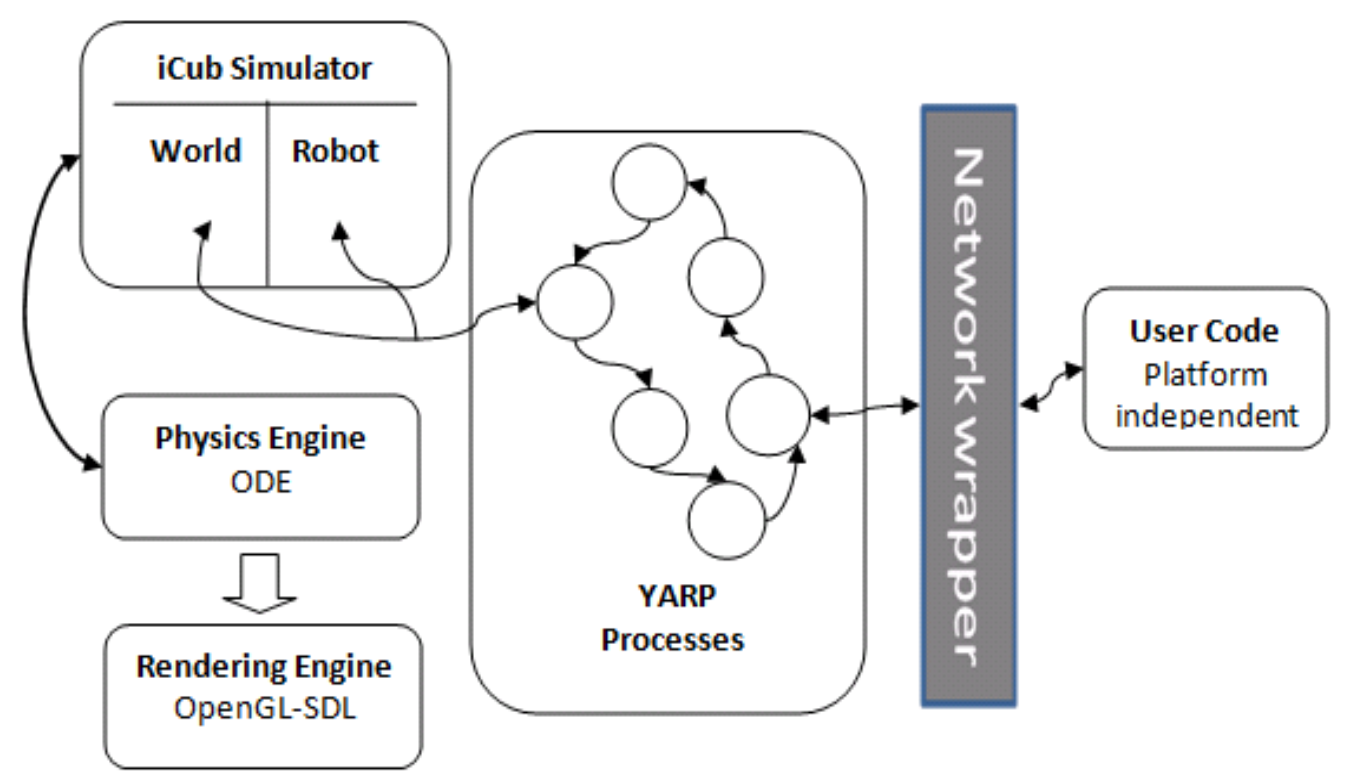
\includegraphics[width=0.95\textwidth]{iCubSim-arch.png} 
\caption{Global view of the software architecture \cite{tikhanoff2008open}.}
\label{fig:iCubSim-arch}
\end{subfigure}
\begin{subfigure}[b]{0.49\textwidth}
\centering
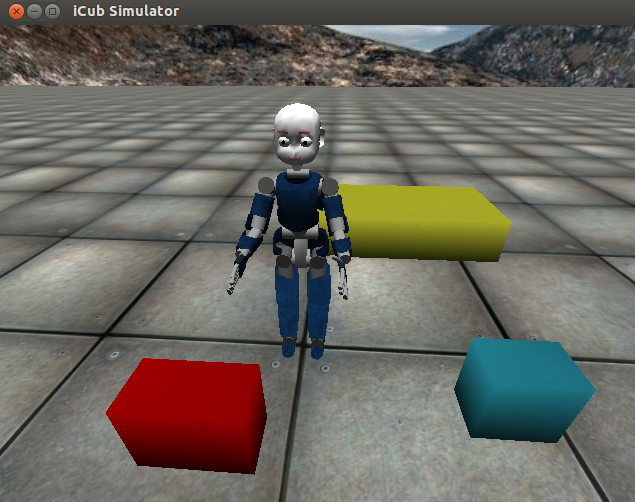
\includegraphics[width=0.95\textwidth]{sim_ode.png}
\caption{A view of the ODE iCubSim simulator.}
\label{fig:iCubSim-view}
\end{subfigure}
\caption{Software architecture and view of the ODE iCub simulator.}
\end{center}
\end{figure*}

\subsection{iCubsim with Gazebo}

One of the shortcomings of the ODE iCub simulator is the way ODE represents rigid-body structures: it represents joints as constraints between bodies. A second class of physics core libraries, such as the ones used in XDE \cite{XDE} and OpenHRP \cite{OPENHRP}, makes use of parametrized rigid-body dynamics representations, where joints are simply part of the robotics structure. These two classes determine not only the way forward/inverse dynamics are computed (the second class benefits from the straightforward computation of quantities useful in robotics, such as Jacobians, mass matrices etc.), but most importantly the way contact forces are computed. The first class considers contacts forces as bilateral/unilateral constraints, which are added to the list of constraints used to describe the joints; then the same solver is used to find the forces for the global system, including contacts and joints. In the second class, on the contrary, only constraints from the contacts are solved, which notably simplifies the problem. This leads to more stable and physically consistent numerical integration results.\\

In order to benefit from alternative physics core libraries and from a widely used, open-source, modular simulation framework, the IIT has developed a new version of its iCub simulator based on Gazebo  \cite{Gazebo}. Gazebo is a multi-robot simulator, developed by the Open-Source Robotics Foundation. It is the official software tool for the Darpa Robotics Challenge and it can rely on Bulletphysics \cite{Bullet} as the physics simulation core. The latest version of Bullet (2.82) relies on efficient dynamics computation algorithms developed by R. Featherstone \cite{Featherstone2007} as well as on the state of the art Mixed Linear Complementarity Problems contact solver developed at INRIA \cite{Siconos}.  A schematic view of the Gazebo iCub simulator software architecture is provided in Fig.~\ref{fig:iCubSimGaz-arch}. A view of the simulator is given in Fig.~\ref{fig:iCubSimGaz-view}.

\begin{figure*}[h]
\begin{center}
\begin{subfigure}[b]{0.49\textwidth}
\centering
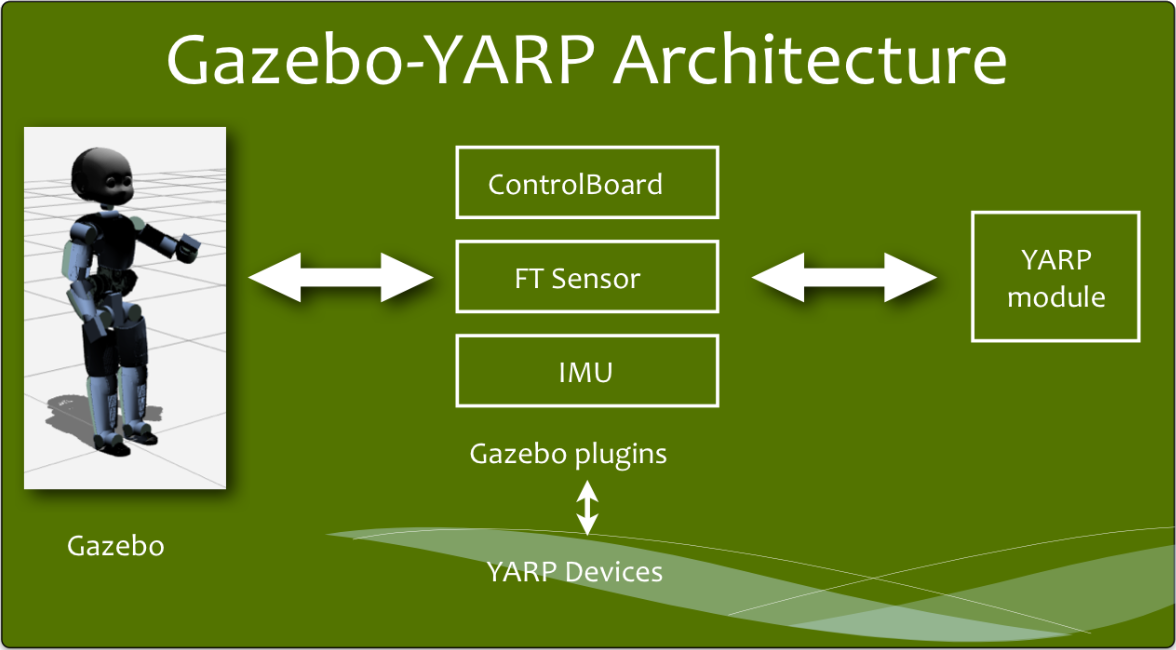
\includegraphics[width=0.95\textwidth]{gazebo-yarp-architecture.png} 
\caption{Schematic view of the software architecture.}
\label{fig:iCubSimGaz-arch}
\end{subfigure}
\begin{subfigure}[b]{0.49\textwidth}
\centering
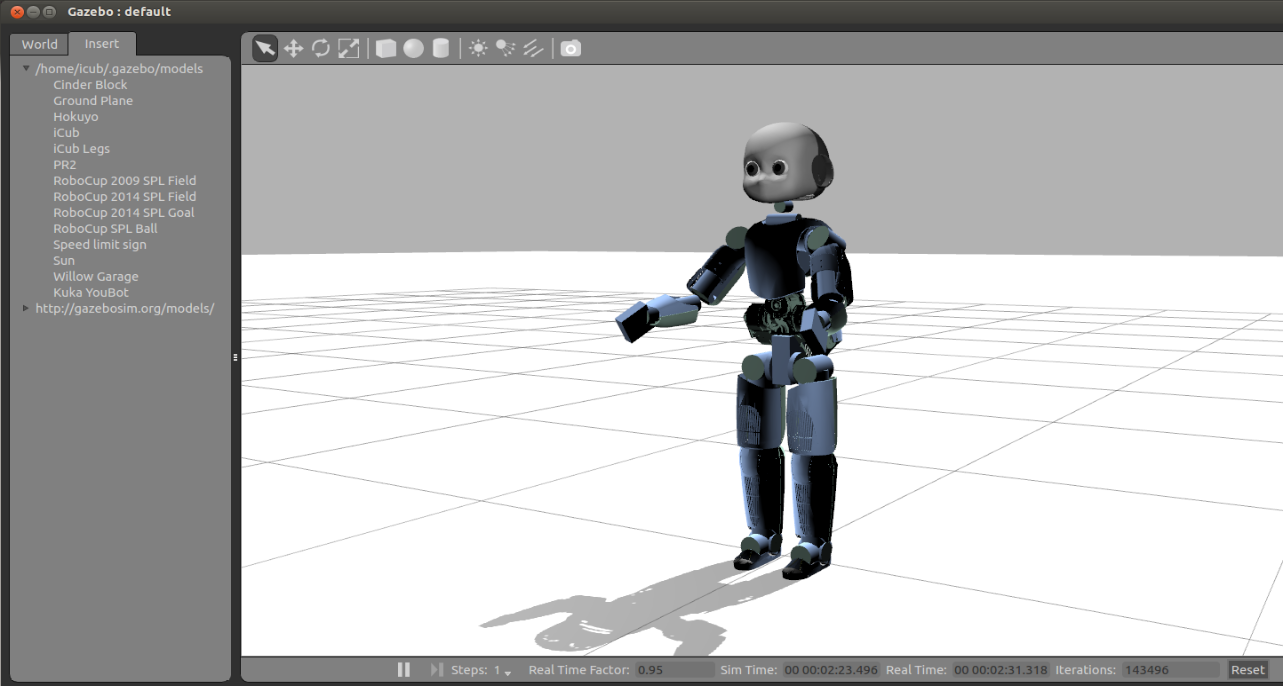
\includegraphics[width=0.95\textwidth]{sim_gazebo.png}
\caption{A view of the Gazebo iCubSim simulator.}
\label{fig:iCubSimGaz-view}
\end{subfigure}
\caption{Software architecture and view of the Gazebo iCub simulator.}
\end{center}
\end{figure*}

\subsection{iCub in XDE}

Based on its past experience with the Arboris-Python\footnote{This simulator was first developed in Matlab by A. Micaelli, researcher at CEA, and then in Python by S. Barth\'el\'emy and J. Salini at UPMC.} dynamics simulator \cite{Arboris-Python} and on its long lasting collaboration with the CEA LIST, UPMC has chosen to explore the possibilities offered by the XDE modular simulation framework \cite{XDE}.\\

XDE is a modular, extensible, component-based simulation framework based on the Orocos \cite{bruyninckx-icra2003} robotics middle-ware and primarily dedicated to interactive simulation and virtual reality applications. XDE is based upon a physics simulation kernel that handles rigid and deformable bodies, in particular cables, multi-body systems with kinematic constraints and intermittent contacts, fluids: liquid, gas or smoke. XDE is equipped with two different proximity computing engines to achieve a precision guaranteed collision detection between objects, even with complex industrial models produced by CAD tools. XDE is based upon widely accepted technologies like Orocos RTT, Python, C++, Ogre, OpenMP, CUDA. It comes with a rigid-body model computation component and its functionalities come with Python wrappers facilitating the rapid prototyping of code.\\

Based on this framework and on the work of Joseph Salini \cite{salini2012} on whole-body controllers for humanoid robots, a model of iCub in XDE has been implemented and several simulations including iCub in whole-body and multi-contact situations have been performed. A view of the simulator including iCub in a whole-body multi-contact situation is given in Fig.~\ref{fig:XDE-view}.

\begin{figure*}[h]
\begin{center}
\centering
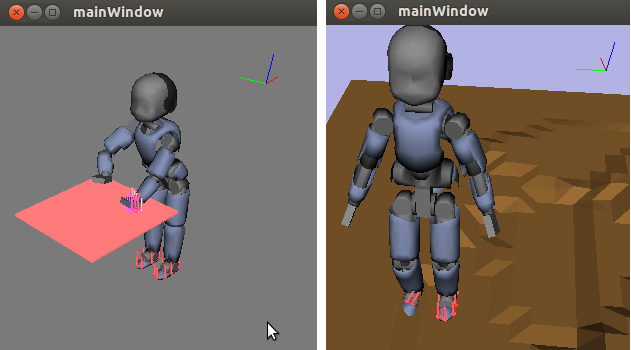
\includegraphics[width=0.6\textwidth]{sim_xde2.png}
\caption{A view of the XDE iCub simulator.}
\label{fig:XDE-view}
\end{center}
\end{figure*}


\subsection{Digital human URDF file generator}

Within the framework of WP2, WP3 and WP4, simulating digital humans using the iCub dynamics simulator (especially in the case where the human-robot interaction is studied) is required. In order to easily generate digital humans of various heights and weights, XDE includes a parametrized digital human model with 45 "actuated" degrees of freedom among which 6 are located in the back. A view of four instances of the same parametrized mannequin with different heights and weights is provided by Fig.~\ref{fig:view-xde-dh}.\\

In order to provide a way to generate URDF \cite{URDF} models of digital mannequins independently from a specific simulator, JSI has developed a software for generating instances of a parametrized digital human (similar to the one present in XDE) as well as to edit the detailed parameters of an existing instance. The user manual of this software is provided in Appendix~\ref{app:dhm urdf}.

\begin{figure*}[h]
\begin{center}
\centering
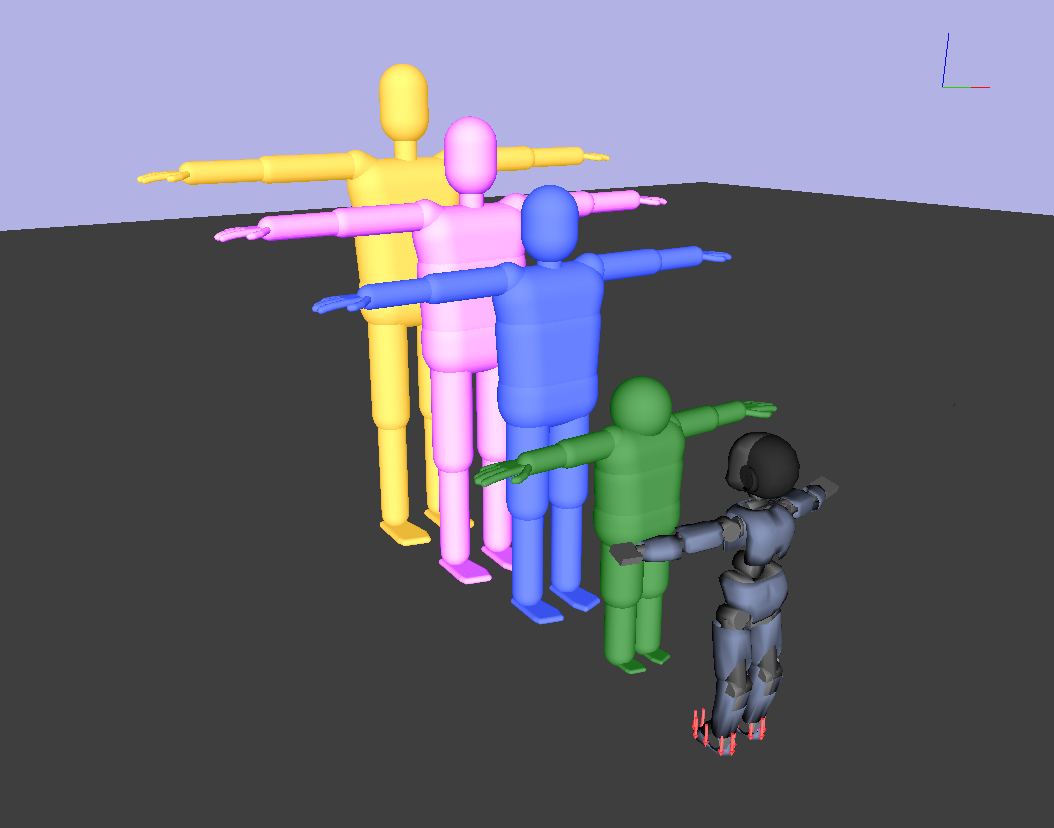
\includegraphics[width=0.7\textwidth]{icub_with_colored_humans.png}
\caption{iCub and four instances of the same parametrized mannequin with different heights and weights in XDE.}
\label{fig:view-xde-dh}
\end{center}
\end{figure*}


\section{Assessment of the proposed simulation solutions}
\label{sec:comparison}

This section describes some preliminary work aiming at quantitatively evaluating the accuracy of the rigid body simulation of the iCub robot in the Gazebo \cite{Gazebo} and XDE \cite{XDE} simulators. In order to perform this comparison, an initial experiment on a real iCub robot is performed. This experiment is used to identify a reasonably accurate model of the friction acting in the real robot so that this model can complete the pre-existing rigid-body model of the robot used for simulation. Friction being a major component of the torques acting on the robot at low velocities, this first phase is needed to ensure that the comparison between the physical and virtual world robot is meaningful. Once this fairly accurate model is obtained, the second stage consists in performing similar experiments on the real robot as well as on its XDE and Gazebo simulated counterparts.

\subsection{Methodology}

The experiment chosen to perform the comparison consists in a free-fall of the right leg of iCub, starting from of a configuration where the leg is stretched horizontally as illustrated by Fig~\ref{fig:exp-gazebo} and Fig.~\ref{fig:exp-xde} respectively in the Gazebo and XDE simulators. A shared URDF model of the iCub robot is used in both simulators.

\begin{figure*}[h]
\begin{center}
\begin{subfigure}[b]{0.49\textwidth}
\centering
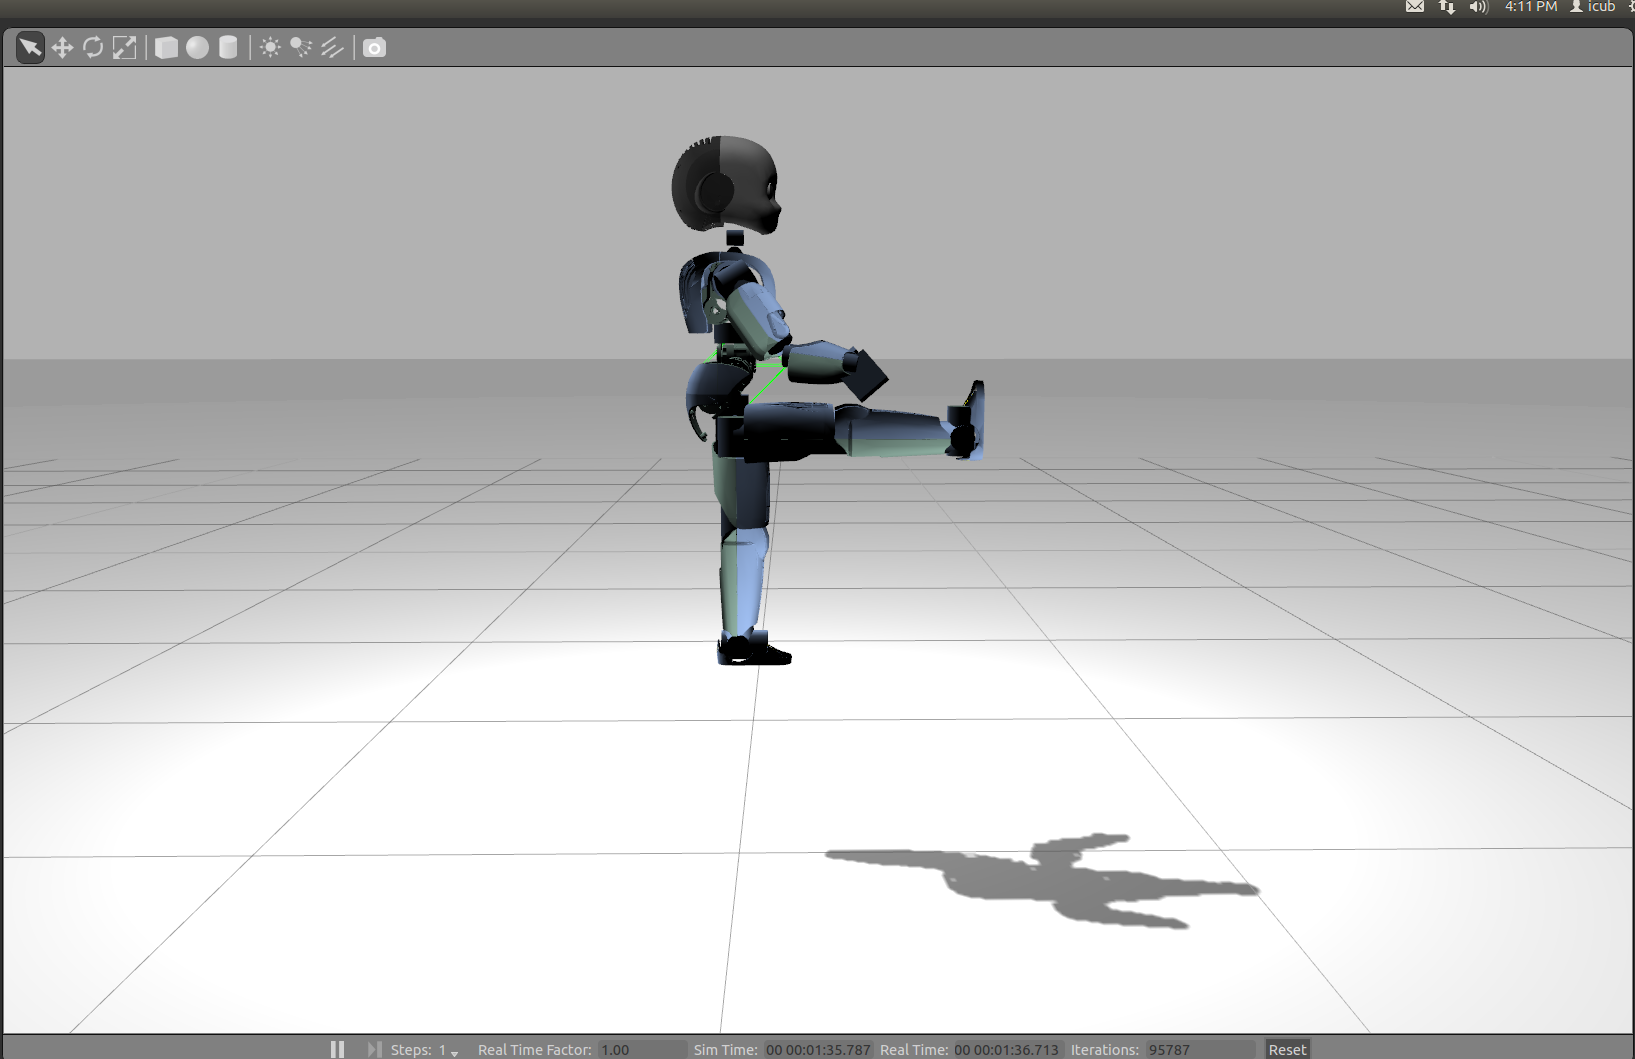
\includegraphics[width=0.95\textwidth]{icub_gazebo_knee.png} 
\caption{Gazebo view.}
\label{fig:exp-gazebo}
\end{subfigure}
\begin{subfigure}[b]{0.49\textwidth}
\centering
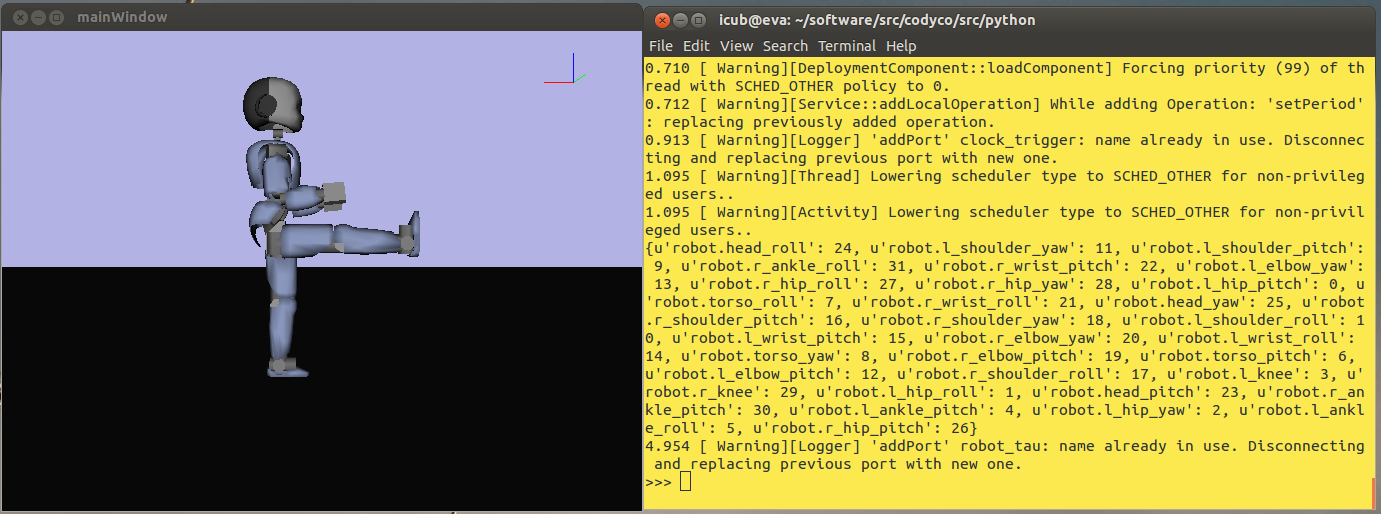
\includegraphics[width=0.8\textwidth]{icub_xde_knee.png}
\caption{XDE view.}
\label{fig:exp-xde}
\end{subfigure}
\caption{iCub Free-falling right leg experiment: initial posture.}
\end{center}
\end{figure*}

While all the dynamics parameters of the robot are computed based on the robot CAD model as well as on the various components data-sheets, a friction model is estimated using a software module\footnote{\href{https://github.com/robotology/codyco/tree/master/src/modules/motorFrictionIdentification}{https://github.com/robotology/codyco/tree/master/src/modules/motorFrictionIdentification}} developed at IIT. The retained friction model $\Gamma_{f,i}$ for joint $i$ can be written as follows
\begin{equation}
	\Gamma_{f,i} = (k_{vp} s(\dot{q}) + k_{vn} s(-\dot{q})) \dot{q} + (k_{cp} s(\dot{q}) + k_{cn} s(-\dot{q})) \mbox{sign}( \dot{q}),
\end{equation}
where $ k_{vp}, k_{cp}, k_{vn}, k_{cn}$ are respectively the viscous and Coulomb friction coefficients for positive joint velocities and the viscous and Coulomb friction coefficients for negative joint velocities. $\dot{q}$ is the joint velocity, $ s(x) $ is the step function ($1$ for $ x>0 $, $0$ otherwise) and $ \mbox{sign}(x) $ is the sign function ($1$ for $ x>0 $, $-1$ for $ x<0 $ , $0$ for $ x=0 $).\\

This model ignores the Stribeck friction regime acting at very low velocities and generating stick-slip behaviours. Still, it can reasonably be used in many applications and presents the advantage of begin linear with respect to the friction coefficients, thus making it rather straightforward to identify using least-squares identification techniques.\\

Two models have been identified: one including both viscous and Coulomb friction components and one including only a hand-tuned/adapted viscous friction component. This hand-tuned coefficient is based on an inverted pendulum model and the obtained value accounts for the mass distribution of the bodies and the observed velocity of the joints on the real robot. Table~\ref{tab:friction-values} summarizes the values obtained by IIT on one of their iCub robot.\\ 

\begin{table*}[h]
\begin{center}
\begin{tabular}{|l|c|c||c|}
\hline 
\backslashbox{Joint}{Coefficient} & Viscous {[}N.m.s{]} & Coulomb {[}N.m{]} & Adapted viscous {[}N.m.s{]}\tabularnewline
\hline 
\multirow{2}{*}{Hip} & $k_{vp} = 0.69212$ & $k_{cp} = 2.64804$ & \multirow{2}{*}{$k_{v}^{\prime} = 93.51401$}\tabularnewline
 & $k_{vn} = 0.68809$ & $k_{cn} = 1.78945$ & \tabularnewline
\hline 
\multirow{2}{*}{Knee} & $k_{vp} = 0.57051$ & $k_{cp} = 2.00711$ & \multirow{2}{*}{$k_{v}^{\prime} = 19.84783$}\tabularnewline
 & $k_{vn} = 0.57482$ & $k_{cn} = 3.21653$ & \tabularnewline
\hline 
\end{tabular}
\caption{Identified friction coefficient for the knee and hip of the iCub robot.}
\label{tab:friction-values}
\end{center}	
\end{table*}

Based on these models and on the real robot experiment, different tests have been performed in both the Gazebo and XDE simulators. It has to be noticed that, both in XDE and Gazebo, viscous friction is intriniscally part of the description of a joint and can thus be integrated implicitly. It is not the case of Coulomb friction. Also, the viscous + Coulomb model exhibits extremely low frictions and thus the retained experiments only compares the real robot motion to the simulated one using the adapted friction model in both simulators.\\

\begin{table*}[h]
\begin{center}
\begin{tabular}{|c|c|c|c|}
\cline{2-4} 
\multicolumn{1}{c|}{} & Real robot & Gazebo & XDE\tabularnewline
\hline 
Real world friction & $A_1$ & - & -\tabularnewline
\hline 
Adapted viscous friction model & - & $B_2$ & $B_3$\tabularnewline
\hline 
\end{tabular}
\caption{Tests performed in the Gazebo and XDE simulators.}
\label{tab:simulator-tests}
\end{center}	
\end{table*}

The joint trajectories of the hip and knee are recorded for comparison. These results are presented in the next subsection.

\subsection{Obtained results}

Figure~\ref{fig:hip} and Figure~\ref{fig:knee} provides plots of the evolution of the hip and knee angle over time in the cases described by Table~\ref{tab:simulator-tests}.\\

The first observation to be drawn from these curves is the large amount of friction faced by the leg joints of the robot. This is a known problem, especially by control people, in most humanoid robots and iCub is similar to them in that sense.\\

The second observation is related to the similarity of the results obtained using both XDE and Gazebo. Some minor differences can be observed but, in this experiment, it is impossible to conclude whether one simulator is more accurate than the other. Indeed, in the process of obtaining these results, IIT and UPMC realized the difficulty to share common robots models, despite the existence of the URDF standard description format. The small difference between the two simulators' results are likely to be due to a mismatch between the used models.\\

Finally, simulating viscous friction is not enough for accurate simulations. This really emphasizes the importance of identification in order to properly close the gap between the real world robot and its simulated counterpart. This is an on-going effort in CoDyCo, especially in WP1, WP3 and WP4.\\

\begin{figure*}[h]
\begin{center}
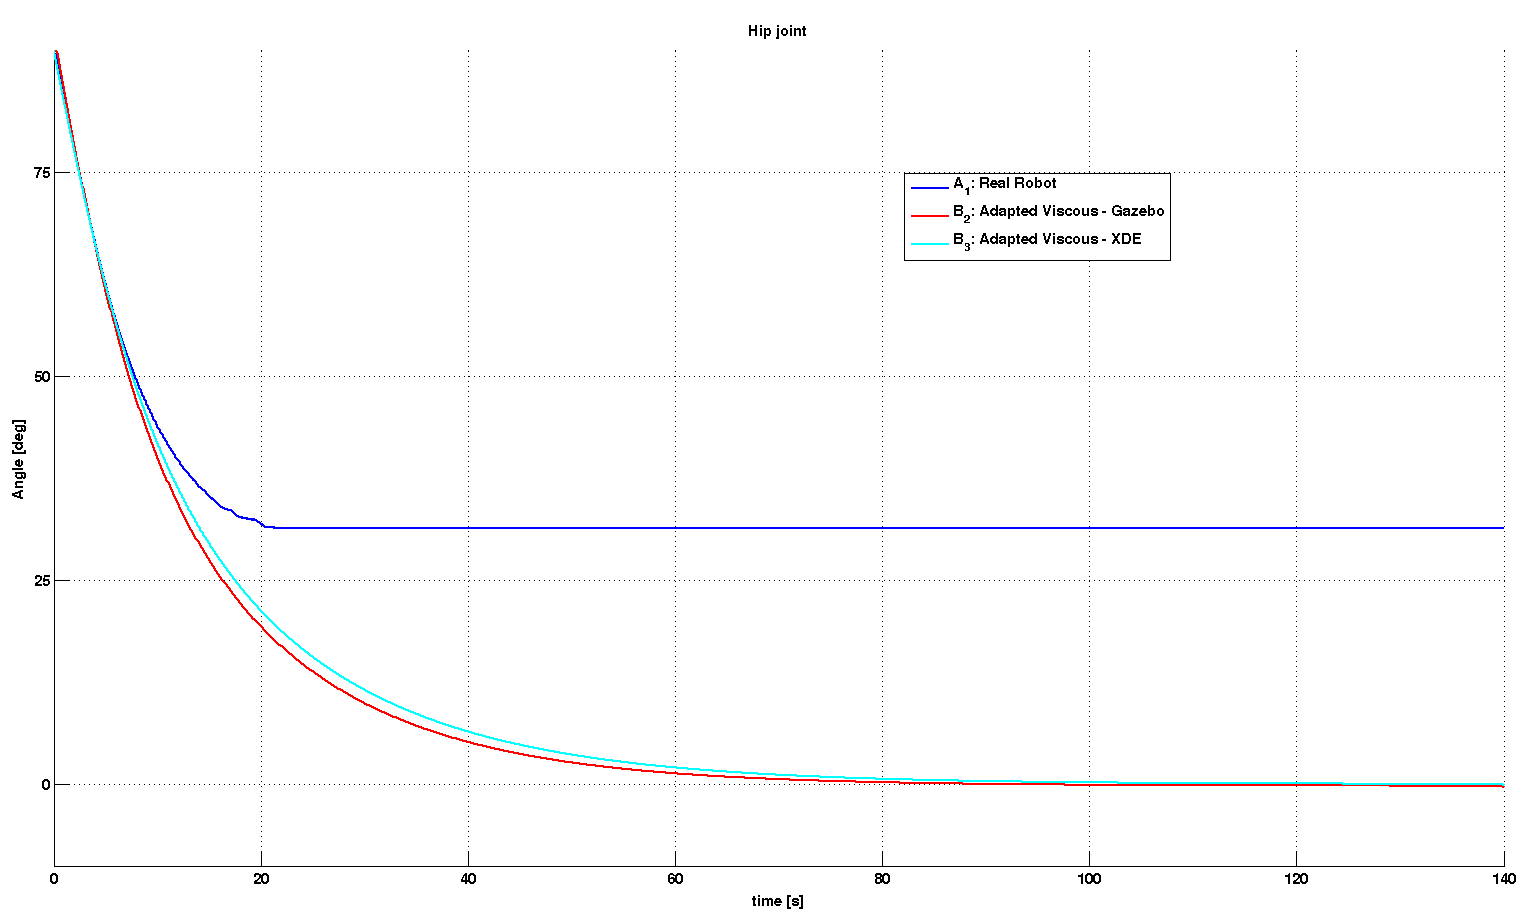
\includegraphics[width=0.95\textwidth]{hip_fig.png}
\caption{Evolution of the hip angle.}
\label{fig:hip}
\end{center}
\end{figure*}

\begin{figure*}[h]
\begin{center}
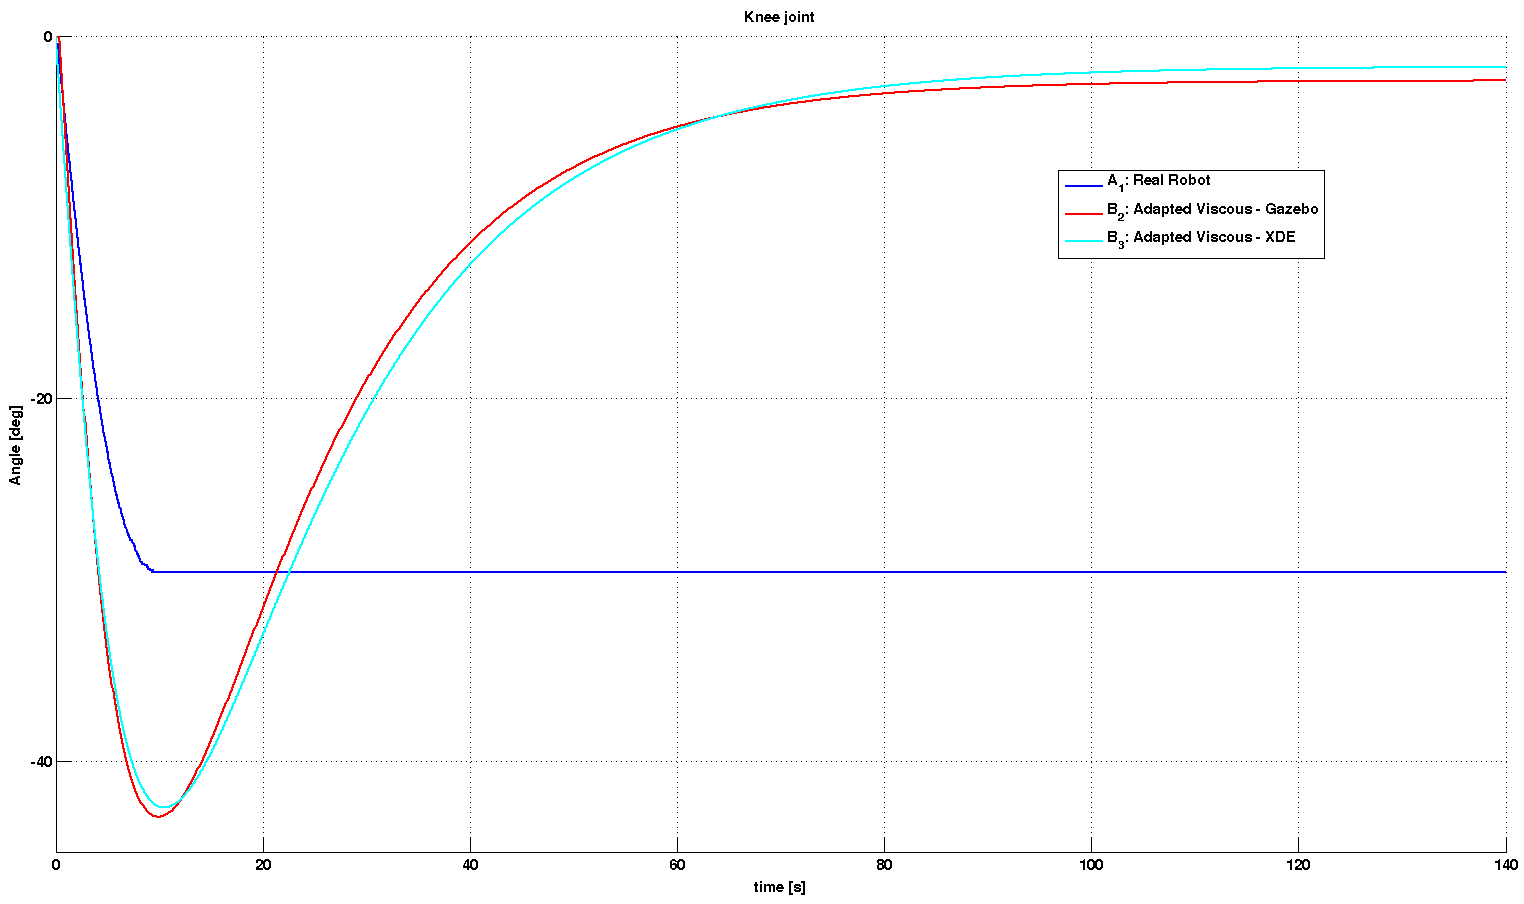
\includegraphics[width=0.95\textwidth]{knee_fig.png}
\caption{Evolution of the knee angle.}
\label{fig:knee}
\end{center}
\end{figure*}



\newpage{}

\phantomsection
\bibliographystyle{IEEEtran}
% argument is your BibTeX string definitions and bibliography database(s)
\bibliography{IEEEabrv,D1.1}
\addcontentsline{toc}{section}{References}

\newpage{}
\begin{appendices}
\section{Robotics simulators survey paper }
\label{app:survey}
\newpage
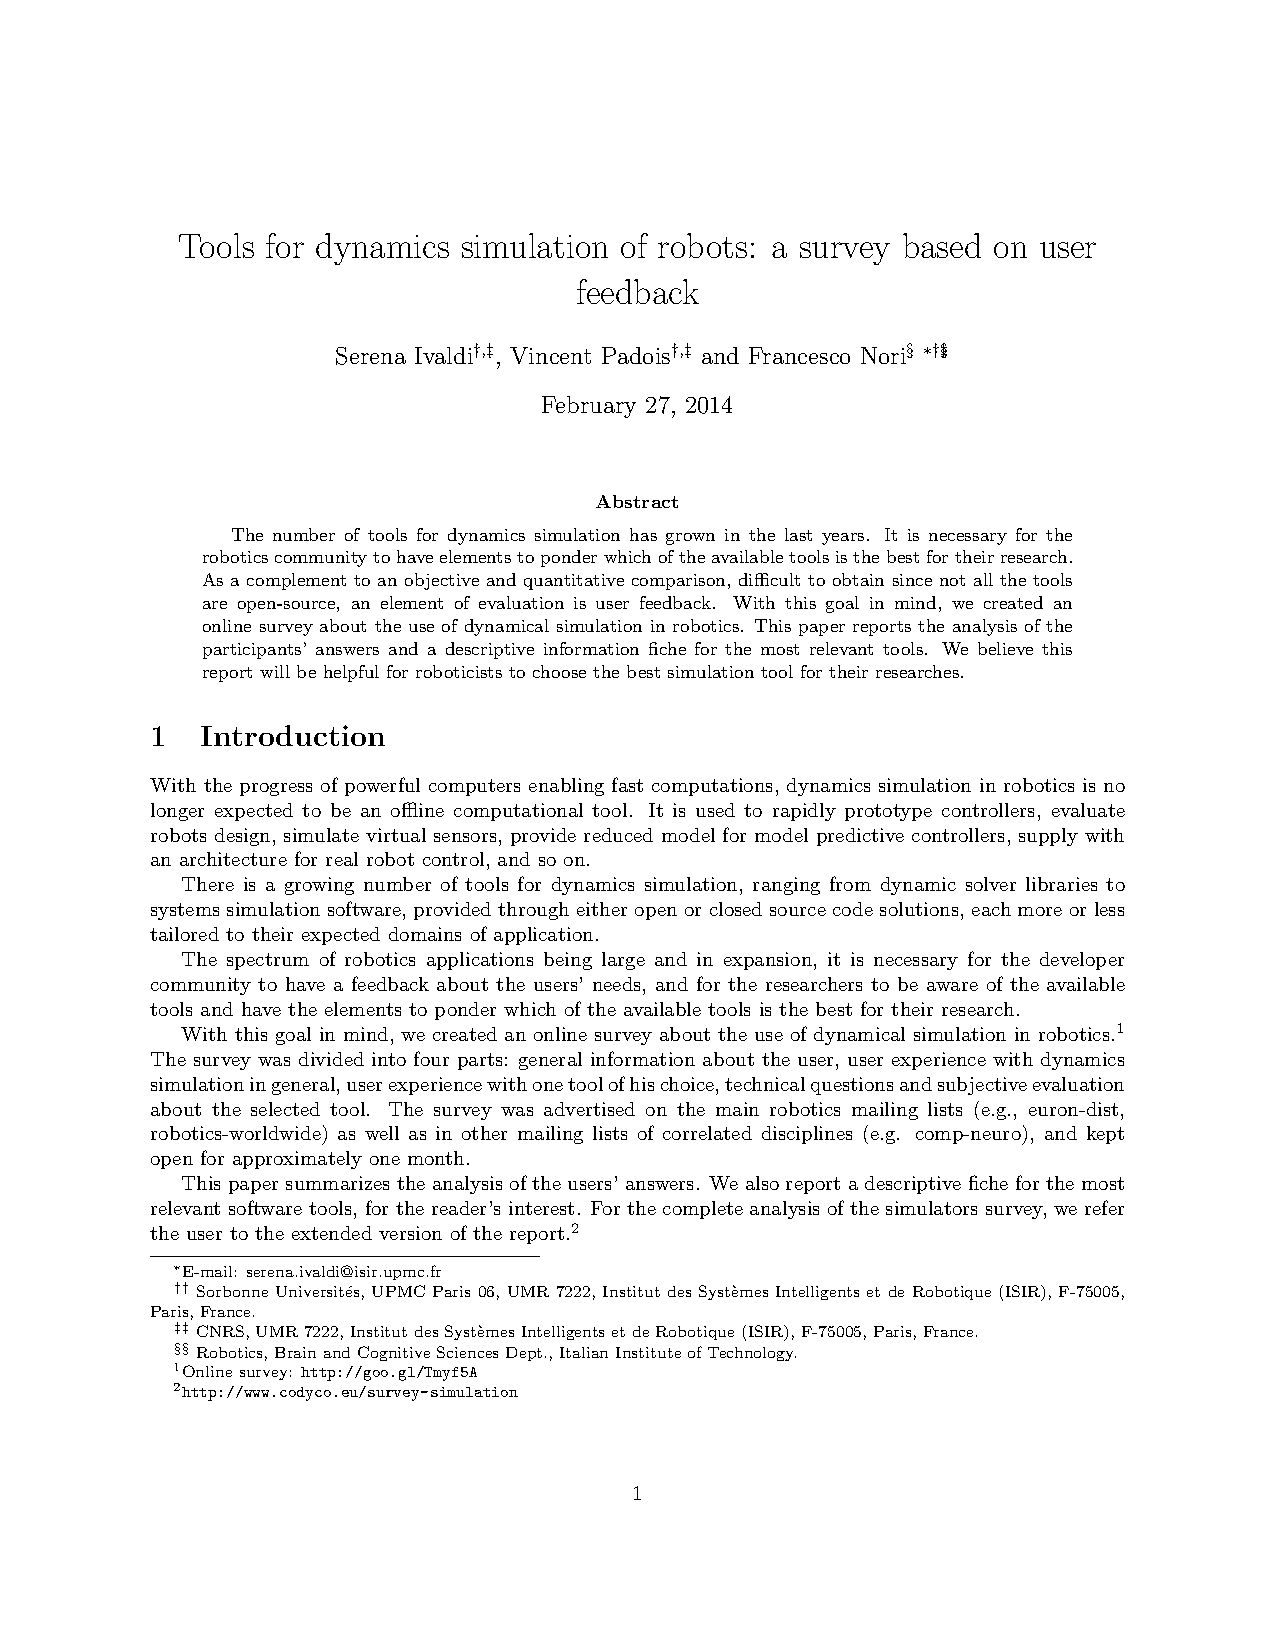
\includepdf[pages={1-16}]{appendix/bare_jrnl_unformatted.pdf}

\section{Technical paper on the digital human URDF file generator}
\label{app:dhm urdf}
\newpage
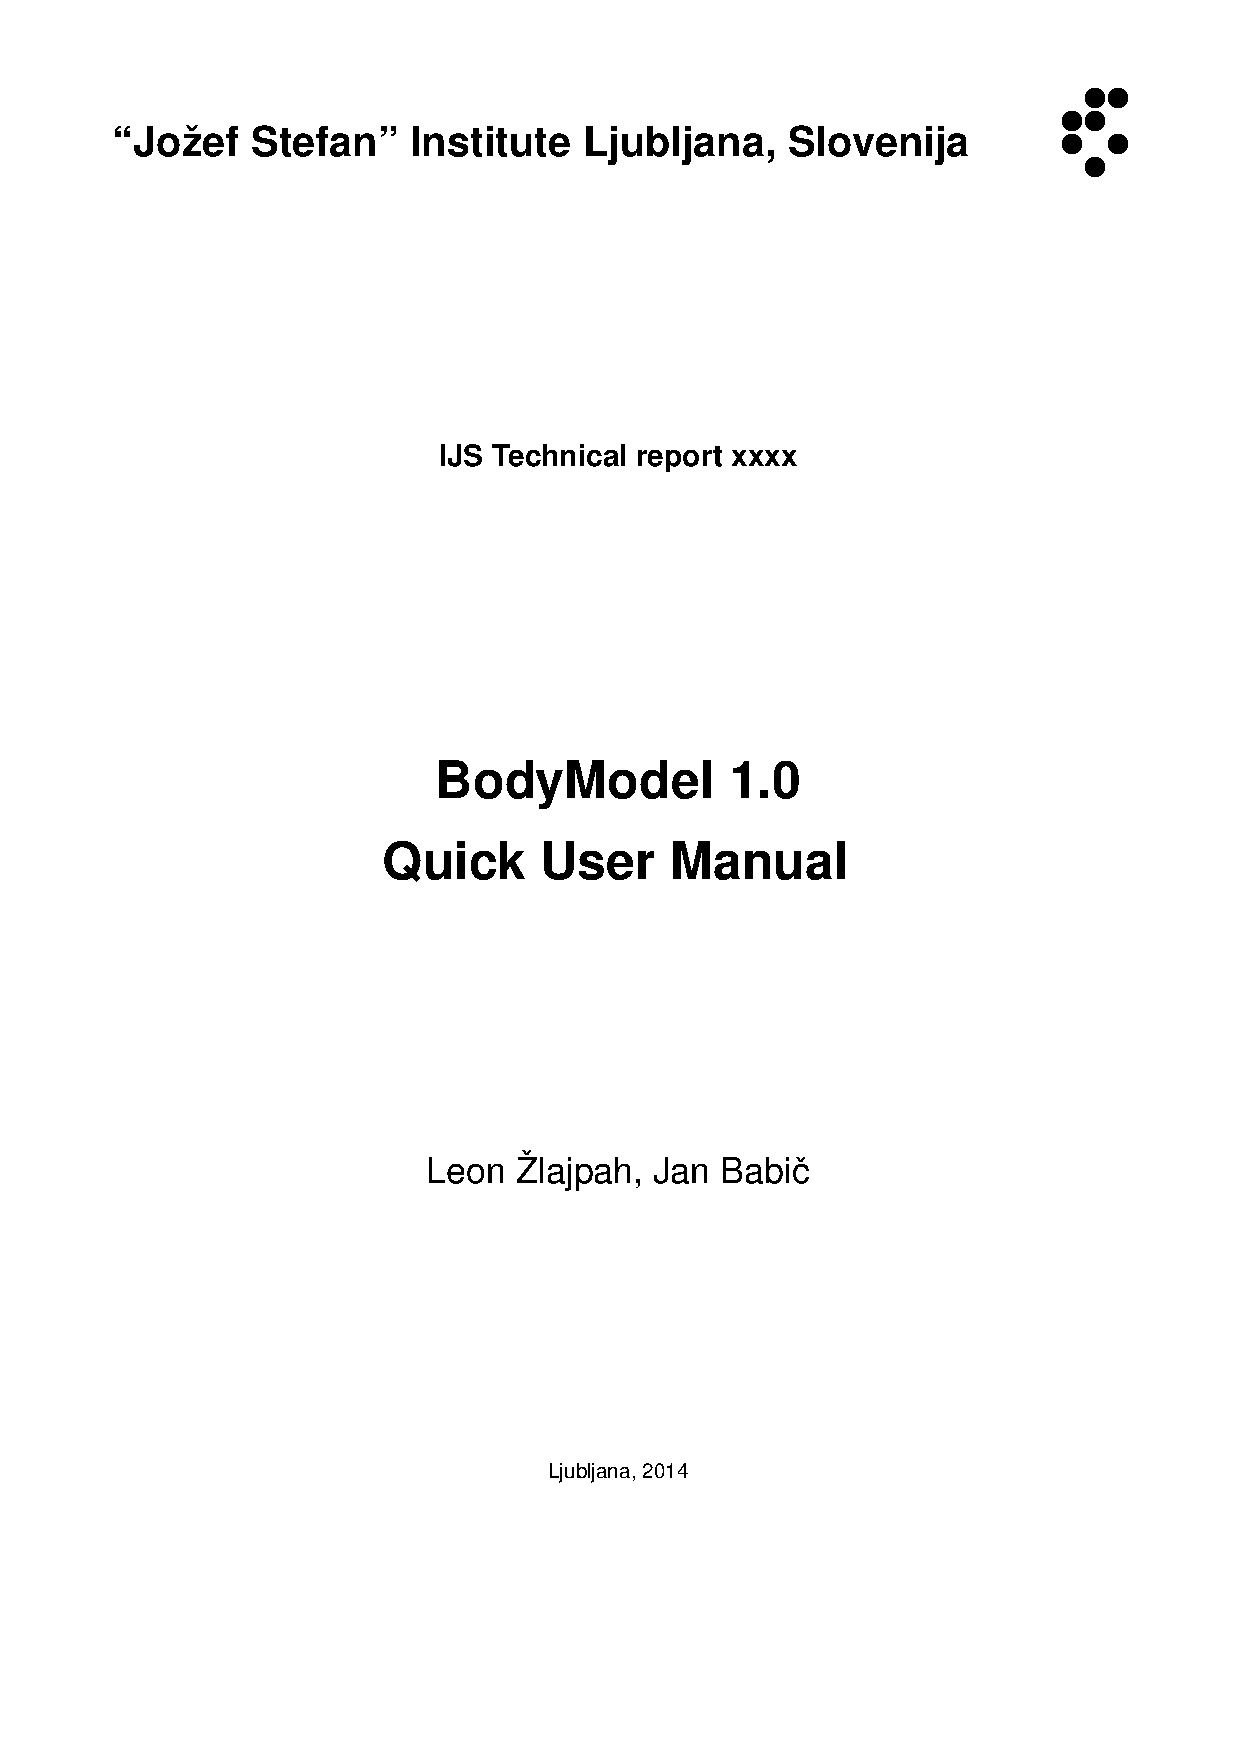
\includepdf[pages={1-13}]{appendix/BodyModel.pdf}
\end{appendices}




\end{document}

%%% Local Variables:
%%% mode: latex
%%% TeX-master: t
%%% save-place: t
%%% End:
